% 原文 pp.194--203
\subsubsectionlink{量子Brown運動の動力学}
調和振動子で中心系を表す量子Brown運動のマスター方程式の一般形(5.25)に戻り、この方程式によって生成される系の時間発展を示そう。この運動は、多くの著者によって詳しく調べられている。ここでは主に、Paz、Habib、Zurek\cite{ref184}の解析に従う。

系の初期波動関数を、コヒーレントな重ね合わせ
\chfiveeq{64}
とする。$\Psi_1(X)$、$\Psi_2(X)$は
\chfiveeq{65}
で与えられるGaussian波束である。ここで$N$は規格化定数、$\delta$は位置空間でのGaussianの幅である。したがって、初め位相空間で対称に位置する二つのGaussian、すなわち、位置が$\pm X_0$で、大きさが同じ逆向きの運動量$P_0$をもつ二つのGaussianの重ね合わせを考えている。

この方法により、位置空間と運動量空間のデコヒーレンスの動力学を調べ、量子Brown運動のデコヒーレンスは運動量の重ね合わせにも作用するのか、それとも位置の重ね合わせだけに作用するのか、この二つの基底でデコヒーレンスの特徴的時間尺度はどう違うのか、といった重要な問いに取り組める。これに答えるため、関心のある二つの極限の場合のデコヒーレンスの動力学を考える\cite{ref184}。最初は、位置だけが離れた（$X_0>\delta$、$P_0=0$）二つのGaussianの重ね合わせ(5.64)、
\begin{equation}
\Psi_{\mathrm{pos}}(X,t=0)=N\left\{\exp\left[-\frac{(X-X_0)^2}{2\delta^2}\right]+\exp\left[-\frac{(X+X_0)^2}{2\delta^2}\right]\right\}
\tag{5.66}
\end{equation}
である。二つ目は、$\Psi_1(X)$と$\Psi_2(X)$の運動量だけが離れた（$X_0=0$、$P_0>1/\delta$）重ね合わせ(5.64)に対応する。
\chfiveeq{67}

% 原文 p.195
\hypertarget{srcpage:195}{}\label{srcpage:195}
いまは座標$X$、$P$で記述する位相空間の描像を用いているので、位置空間の密度行列$\rho_{\mathrm S}(X,X')=\Psi(X)\Psi^*(X')$のWigner表示$W(X,P)$［(2.132)参照］に移るのが便利である。Gaussian波束のWigner表示は、やはり$(X,P)$平面に局在したGaussianなので、初期状態(5.64)に対応するWigner関数は、かなり容易に計算できる。二つの直接項$\Psi_1(X)\Psi_1^*(X')$、$\Psi_2(X)\Psi_2^*(X')$のWigner表示は、次の形をもつことが示せる\cite{ref184}。
\chfiveeq{68}
非対角の干渉項$\Psi_1(X)\Psi_2^*(X')$、$\Psi_2(X)\Psi_1^*(X')$の寄与は、Wigner表示では
\begin{equation}
W_{\mathrm{int}}(X,P,t=0)=2N^2\delta^2\exp\left[-\frac{X^2}{\delta^2}-\delta^2P^2\right]\cos[2X_0P+2P_0X]
\tag{5.69}
\end{equation}
となる。したがって、初期状態(5.64)の完全なWigner関数は
\chfiveeq{70}
である。この関数を、位置だけ、運動量だけが離れている二つの極限、すなわち$\Psi_{\mathrm{pos}}(X,t=0)$［(5.66)参照］と$\Psi_{\mathrm{mom}}(X,t=0)$［(5.67)参照］について、図5.4の最上段に示す。二つの「古典的な」直接ピークが、それぞれ$X$軸と$P$軸に沿って局在している様子が、はっきりわかる（2.15.2節の一般的議論も参照）。また、これらのピークの間には、特徴的な振動模様が見える。その「山」と「谷」は、ピークを結ぶ軸、すなわち隔たりが生じている変数に対応する軸に平行である。(5.69)から明らかなように、振動の波数は、隔たり$X_0$と$P_0$によって直接決まる［(2.135)も参照］。

次に、Wigner表示で表したBorn--Markovマスター方程式(5.29)で与えられる、Wigner関数(5.70)のその後の時間発展を調べよう。ここでは導出の詳細に立ち入らないが、時間発展後のWigner関数も、やはり
\chfiveeq{71}
という形に書け、直接項と干渉項は
\chfiveeq{72a_72b}
で与えられることが示せる\cite{ref184}。

% 原文 p.196
\hypertarget{srcpage:196}{}\label{srcpage:196}
\begin{figure}[htbp]\centering
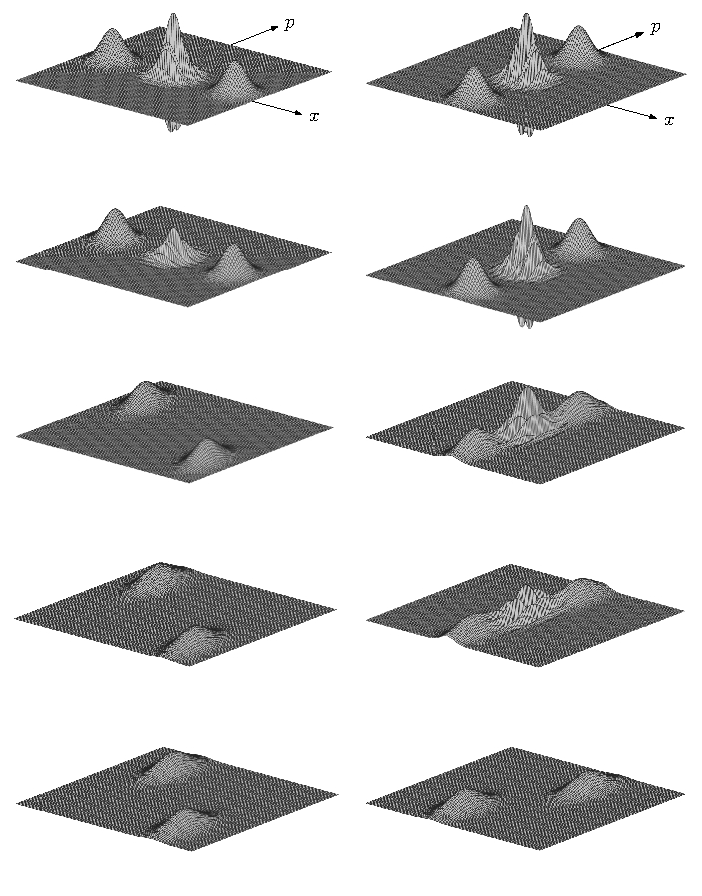
\includegraphics[width=.9\linewidth]{figures/ch05_fig04.pdf}
\caption{Paz、Habib、Zurek\cite{ref184}が調べた、Wigner描像での二つのGaussian波束の重ね合わせの時間発展。左列は、初期波束が位置だけ離れている場合、右列は、運動量だけ離れた波束の重ね合わせの動力学に対応する。二つの波束の干渉は、直接ピーク間の振動で表される。環境との相互作用は、この振動を減衰させ、この過程がデコヒーレンスを表す。ただし、この減衰は、二つの初期条件に対して異なる時間尺度で起こる。}\label{fig:5.4}
\end{figure}

% 原文 p.197
\hypertarget{srcpage:197}{}\label{srcpage:197}
ここで係数$\delta_1$、$\delta_2$、$X_{\mathrm c}$、$P_{\mathrm c}$、$\beta$、$A_{\mathrm{int}}$、$\kappa_x$、$\kappa_p$は、一般に時間依存であり、初期値は、［(5.72)と(5.68)、(5.69)を比較］
\chfiveeq{73a_73b_73c}
である。量子Brown模型の厳密解、すなわち上の扱いで用いたBorn--Markov近似を行わない解（後の5.2.7節参照）から得られる、これらの係数の具体的な、ただし非常に複雑な一般式は、環境のスペクトル密度の任意の選択に対して、Paz、Habib、Zurek\cite{ref184}が与えている。Born--Markov近似に注目し、スペクトル密度を特定の形に選べば、より簡単で具体的な表式が得られる。

いずれにせよ、ここでは係数の正確な形には、これ以上立ち入らない。代わりに、(5.71)、(5.72)が記述するWigner関数の時間発展の、十分な定性的描像を得よう。この発展は、二つの極限的な初期状態(5.66)、(5.67)について、図5.4に示されている。どちらの初期条件でも、環境との相互作用によって、波束の量子干渉を表す振動が抑制される。しかし、このデコヒーレンスが起こる時間尺度は、大きく異なる。初め位置だけ離れた二つの波束の重ね合わせ(5.66)は、運動量の重ね合わせ(5.67)より、はるかに速くデコヒーレンスを起こす。実際、後で詳しく解析するように、最初の場合、デコヒーレンスの時間尺度は、系の緩和時間尺度や力学的時間尺度に、事実上依存しない。これに対し、運動量の重ね合わせという二つ目の場合、量子干渉は、系の固有の運動、すなわち自己Hamiltonianが定める時間尺度で減衰する。

この観察は、かなり容易に説明できる。相互作用Hamiltonianは、系の位置に陽に依存する。これは、環境が位置を直接監視し、位置基底に強く速いデコヒーレンスをもたらすことを意味する。一方、系の運動量は相互作用Hamiltonianに現れないため、環境から直接監視されない。したがって運動量のデコヒーレンスは、位置の監視と、その結果の位置のデコヒーレンスを通じ、間接的にしか起こりえない。

% 原文 p.198
\hypertarget{srcpage:198}{}\label{srcpage:198}
波束が初め運動量だけ離れている場合、状態(5.67)は、すでに位置についてよく局在している。したがって、系の位置の環境監視は、この状態をさらに位置局在させることはできず、重ね合わせ(5.67)は初め、環境監視、ひいてはデコヒーレンスに敏感ではない。

しかし、二つの直接ピークに付随する逆向きの運動量$\pm P$が、そのピークを$X$の逆方向へ移動させるので、力学的時間尺度で、この重ね合わせは位置の重ね合わせへと発展する（図5.4の右列参照）。すると、状態は位置の環境監視に敏感になり、それが振動の減衰をもたらす。このことは、相互作用Hamiltonianに運動量項がないのに、なぜ運動量のデコヒーレンスが起こるのか、そして、なぜそれが、位置のデコヒーレンス、すなわち環境が直接監視する量のデコヒーレンスの、はるかに短い時間尺度ではなく、力学的時間尺度で起こるのかを説明する。以下では、Wigner関数(5.71)の直接項(5.72a)と干渉項(5.72b)に現れる量の時間依存性を解析し、この議論をより正確にする。

まず、直接項$W_{1,2}(X,P,t)$で記述するGaussianピークの運動を見よう。これらのピークは、$X(t)=\pm X_{\mathrm c}(t)$、$P(t)=\pm P_{\mathrm c}(t)$という「古典的」軌道をたどる。この軌道はスペクトル密度の具体的選択には依存するが、環境の温度には依存しない。Gaussianピークの幅は、$\delta_1$（位置幅）と$\delta_2$（運動量幅）で与えられ、環境の存在によって時間とともに変化する。また、環境はGaussianの形を歪ませ、その程度は係数$\beta$で定量化される。幅$\delta_{1,2}$と歪み$\beta$は、いずれも環境のスペクトル密度と温度に依存する。

デコヒーレンスの議論で最も興味があるのは、干渉項$W_{\mathrm{int}}(X,P,t)$［(5.72b)参照］であり、これは波束$\Psi_1(x)$と$\Psi_1(x)$の干渉を特徴づける振動を表す。まず、$X$軸、$P$軸に沿った振動の、温度に依存する波数$\kappa_x$、$\kappa_p$が、環境との相互作用で変わる。デコヒーレンスに最も関係する量は$\exp(-A_{\mathrm{int}})$であり、後で見るように、これは振動の減衰、したがってデコヒーレンスを記述する。この項は干渉縞の可視度を定量化すると解釈できる。$\exp(-A_{\mathrm{int}})$は、$X=P=0$で最大となる干渉項$W_{\mathrm{int}}(X,P)$と、$X=\pm X_{\mathrm c}$、$P=\pm P_{\mathrm c}$で最大となる直接項$W_{1,2}(X,P)$の、ピークの比に等しいからである。
\begin{equation}
\exp(-A_{\mathrm{int}})=\frac12\frac{W_{\mathrm{int}}(X=0,P=0)}{[W_1(X=X_{\mathrm c},P=P_{\mathrm c})W_2(X=-X_{\mathrm c},P=-P_{\mathrm c})]^{1/2}}.
\tag{5.74}
\end{equation}

% 原文 p.199
\hypertarget{srcpage:199}{}\label{srcpage:199}
この解釈から、$\exp(-A_{\mathrm{int}})$は、しばしば「干渉縞可視度関数」と呼ばれる。量$A_{\mathrm{int}}$は、次で与えられることが示せる\cite{ref184}。
\chfiveeq{75}
ここに現れる量は、すべて陽に時間依存すると理解する。時刻$t=0$では、$\delta_1=\delta_2=\delta$、$\kappa_x=P_0$、$\kappa_p=X_0$［(5.73)参照］なので、$A_{\mathrm{int}}=0$である。その後の時刻$t>0$では、$A_{\mathrm{int}}$は増大するが、常に、時間に依存しない漸近的な最大値
\chfiveeq{76}
によって上から抑えられる。実際、量子Brown運動のマスター方程式から、$A_{\mathrm{int}}$の具体的な運動方程式を導ける。結果は\cite{ref184}
\chfiveeq{77}
である。$D$と$f$は、Born--Markov近似での通常拡散係数と異常拡散係数である（Redfield方程式または厳密なマスター方程式\cite{ref219}を用いれば、これらは陽に時間に依存する。5.2.7節も参照）。

(5.77)は、$A_{\mathrm{int}}$の時間発展、したがって干渉項が抑制される動力学が、いくつかのパラメータに依存することを示す。まず、$A_{\mathrm{int}}$の時間変化は、拡散係数$D$、$f$に陽に直接依存するが、マスター方程式(5.25)の運動量減衰（摩擦）係数$\gamma$にも、繰り込まれたHamiltonian $\hat H'_{\mathrm S}$による自由発展にも、直接は依存しない。ただし、(5.77)の$\kappa_x$、$\kappa_p$の運動は$\gamma$と$\hat H'_{\mathrm S}$に依存するため、$A_{\mathrm{int}}$の時間発展も、これらから間接的に影響を受ける。

一方、後で見るように、$\gamma$と$\hat H'_{\mathrm S}$の間接的影響は、通常、拡散係数に対する直接的依存性と比べて非常に弱い。このことは、すでに重要な結論を示唆する。多くの場合、$A_{\mathrm{int}}$の発展、したがってWigner関数の振動項の抑制は、$\gamma$で定まる緩和時間尺度と、$\hat H'_{\mathrm S}$で決まる力学的時間尺度に、本質的に依存しない時間尺度で起こる。

(5.77)の右辺の第1項$4D\kappa_p^2$は非負なので、通常拡散係数$D$は、常に干渉項の抑制、したがってデコヒーレンスに対応する。(5.72b)より、$\kappa_p$は、運動量方向に沿ったWigner振動の波数を定量化する。(5.77)から明らかなように、第2項の符号は一定ではなく、$\kappa_x$と$\beta\kappa_p$の兼ね合いに依存する。したがって、異常拡散係数$f$は、干渉の抑制を助ける役割から、この抑制に対抗する役割へと変わることがある。

% 原文 p.200
\hypertarget{srcpage:200}{}\label{srcpage:200}
(5.77)が与える$A_{\mathrm{int}}$の時間発展の決定的な特徴は、初期条件、特に初期の隔たり$X_0$、$P_0$への直接的依存性である。この依存性は、時刻$t=0$で$\kappa_x=P_0$、$\kappa_p=X_0$となる係数$\kappa_x$、$\kappa_p$を通じて入る［(5.73b)参照］。以下で見るように、この依存性が、前述の、位置と運動量のデコヒーレンスの時間尺度の大きな違いを生む（図5.4も参照）。

まず、初期状態が、位置空間だけで離れた二つのGaussianの重ね合わせである極限(5.66)に注目しよう。$t=0$で$\kappa_p=X_0$なので、$A_{\mathrm{int}}$の発展方程式(5.77)の通常拡散項$4D\kappa_p^2$は、直ちに干渉の減衰に寄与する。

上の5.2.4節で論じた、高温のOhmic環境という簡単なCaldeira--Leggettの場合について、(5.77)の$A_{\mathrm{int}}$の時間依存性を調べよう。ここでは、異常拡散係数$f$は通常拡散係数$D$に比べて無視でき、$D$は$2M\gamma_0k_{\mathrm B}T$で近似できる［(5.51)参照］。さらに、干渉縞は時間とともにほとんど移動しない、すなわち$\kappa_p$の時間依存性を無視し、その初期値$X_0$で置き換えられるという、簡単化の仮定を置こう。この仮定のもとで、(5.77)は容易に解け、
\chfiveeq{78}
または、熱的de Broglie波長$\lambda_{\mathrm{dB}}=1/\sqrt{2Mk_{\mathrm B}T}$を用いて、
\chfiveeq{79}
を得る。したがって、Wigner関数の振動は、デコヒーレンス率
\chfiveeq{80}
で指数関数的に減衰する。$\Delta X$は位置空間のコヒーレントな隔たりである。こうして、Caldeira--Leggettの場合のデコヒーレンス率についての先の結果(5.61)を再び得る。

次に、Gaussianの重ね合わせが、初めは運動量だけ離れた、すなわち$X_0=0$である状況(5.67)を考えよう。$t=0$で$\kappa_p=0$なので、初めは$\mathrm dA_{\mathrm{int}}/\mathrm dt=0$となる。すなわち、$\kappa_p=0$がゼロから離れ始めるまで、$A_{\mathrm{int}}$は初期値ゼロにとどまり、この初期段階ではデコヒーレンスが起こらない。弱く減衰する系では、$\kappa_p$は$\kappa_p(t)\propto X_{\mathrm c}(t)$のように発展し、その値が直接ピークの軌道に従うことを示せる\cite{ref184}。したがって、$\kappa_p$の増加は$X_{\mathrm c}$の変化と結びつく。$X_{\mathrm c}$は初期値ゼロから始まり、力学的時間尺度で発展する。

% 原文 p.201
\hypertarget{srcpage:201}{}\label{srcpage:201}
すると、(5.77)の拡散項が$A_{\mathrm{int}}$に作用できるようになり、$A_{\mathrm{int}}$が正となって、Wigner干渉項$W_{\mathrm{int}}(X,P,t)$［(5.72b)参照］の振動が抑制される。

したがって、運動量だけ離れたGaussian波束の重ね合わせでは、デコヒーレンスは、二つの異なる時間尺度に関係する。第一は、位置の重ね合わせが生成される比較的遅い力学的時間尺度である。すなわち、$X_{\mathrm c}$が初期値ゼロから十分離れ、環境による系の位置の監視が作用できるようになる時間尺度である。第二に、位置の重ね合わせが動的に作られると、それは位置空間の重ね合わせのデコヒーレンス時間尺度（例えば高温Ohmic環境では(5.80)）で、急速にデコヒーレンスを起こす。したがって、運動量のデコヒーレンス率は、常に系の力学的発展の速さによって制限される。これは、運動量のデコヒーレンスに関係する時間尺度が、力学的時間尺度だけであることを意味する。この解析は、位置空間に比べて運動量空間のデコヒーレンスが、はるかに遅いという最初の直観的説明を、厳密に支える。

環境との相互作用によって選び出される優先状態、すなわち指針状態は、結局どのようなものだろうか。これに答えるため、調和振動子系の縮約密度行列$\hat\rho_{\mathrm S}$の純度$\varsigma=\operatorname{Tr}\hat\rho_{\mathrm S}^2$［(2.30)参照］の変化を計算できる。この変化はBorn--Markovマスター方程式(5.25)から求められる。ここでは、運動量減衰項$\gamma$の影響を無視する。この項は常に、密度行列の形にまったく依存しない、純度の非物理的な時間増加をもたらすことが示せるからである\cite{ref016}。この項の省略は、弱減衰の極限、すなわち「不足減衰」の調和振動子の場合には十分正当化できる。また、高温極限では適切である（5.2.4節参照）ため、異常拡散項も無視する。この仮定のもとで、純度の瞬間的変化は\cite{ref086}
\chfiveeq{81}
となる。$\Delta X^2(t)=\langle\hat X^2\rangle_t-\langle\hat X\rangle_t^2$は、位置空間の分散である。したがって、この空間分散を最小にすれば、純度の瞬間的減少、したがってデコヒーレンスの大きさも最小となる。すなわち、瞬間的な指針状態は、位置について完全に局在したものであろう。この結果は、環境が系の位置を直接監視することから、予想できたかもしれない。

しかし、自己Hamiltonian(5.23)で与えられる調和振動子系の固有の発展も、重要な役割を果たす。実際、調和振動子についてよく知られているように、一周期$T=2\pi/\Omega$の間に、位置と運動量は役割を入れ替える。

% 原文 p.202
\hypertarget{srcpage:202}{}\label{srcpage:202}
系のHamiltonianが位置変数と運動量変数についてもつこの対称性は、位相空間で非対称に局在する状態（例えば位置にはよく局在するが、運動量には完全に非局在化した状態）が、系のHamiltonianによる時間発展で大きく変わることを意味する。

この議論を正確にするため、純度の瞬間的変化(5.81)を調べる代わりに、調和振動子系の完全な一周期$t=0\ldots T$にわたって平均した、純度の変化を見よう。この平均変化は、次で与えられることが示せる\cite{ref015,ref084}。
\chfiveeq{82}
ここで$\Delta X^2\equiv\Delta X^2(0)$、$\Delta P^2\equiv\Delta P^2(0)$は、初期時刻$t=0$での位置と運動量の分散である。異常拡散項$f$は、(5.81)のようにあらかじめ無視しなくても、一周期でその影響が平均して消えるため、(5.82)に現れない。

(5.82)は、不確定性関係が課す$\Delta X\Delta P\geq1/2$の制約（本章を通じて$\hbar\equiv1$としたことを思い出そう）のもとで、右辺の括弧内を最小にするように$\Delta X^2$、$\Delta P^2$を選べば、純度の平均減少、したがってデコヒーレンスの大きさが最小になることを示す。純度の減少(5.82)を最小にする選択は
\chfiveeq{83}
であるとわかる。したがって、量子Brown運動で環境により超選択される指針状態は、位置と運動量の両方でよく局在する、最小不確定性Gaussian、すなわちコヒーレント状態である。これを最初に示したのはZurek、Habib、Paz\cite{ref086}である（文献\cite{ref084,ref223,ref224,ref225,ref226}も参照）。

もちろん、量子力学は位相空間での完全な局在化を禁じるが、環境との相互作用で選ばれるコヒーレント状態は、「これ以上よくはできない」位相空間局在を表す。したがって、このコヒーレント状態を、位相空間の古典的な一点という理想概念の、量子版とみなせる。縮約密度行列が記述する、最小不確定性Gaussian波束の非真正アンサンブルを、時間を追って同定し直すことで、位相空間における粒子の準Newton的な軌道を取り戻せる。

厳密にいえば、量子Brown運動の指針状態がコヒーレント状態であるという上の導出は、弱く減衰する調和振動子の仮定に基づく。しかし、強減衰領域でも結論は大きく変わらず、主な違いは、運動量より位置の局在が、より強く優先されることである\cite{ref227}。さらにEisert\cite{ref106}は、熱浴に結合した自由量子粒子の場合、最小不確定性Gaussian状態の環境誘起超選択は、完全に一般的であることを示した。

% 原文 p.203
\hypertarget{srcpage:203}{}\label{srcpage:203}
すなわち、任意の浴温度、系と環境の結合強度、環境スペクトル密度に対して、そのようなコヒーレント状態への厳密なデコヒーレンスが起こる。

最後に、環境の振動数が系の固有振動数に比べて非常に小さい極限についても、量子Brown運動の優先状態の環境誘起超選択を調べられる。この「遅い」環境の極限は、5.2.4節のCaldeira--Leggett模型の状況とは反対であり、デコヒーレンスの「量子極限」に対応する（2.8.2節参照）。PazとZurek\cite{ref103}は、標準的な量子Brown運動模型の変種、すなわちスカラー場と相互作用する粒子を考え、この極限では、縮約密度行列の純度の減少が、系のエネルギー固有状態、すなわち自己Hamiltonianの固有状態について最小となることを見いだした。したがって、それらが系の指針状態として出現する。この結果は、2.8節の一般的な議論と一致する。
